\subsection{Artificial Neural Network}
An Artificial Neural Network (ANN) have been trained to solve the regression problem. For ease of comparison with the linear regression a 10-fold cross validation has been used as well. The network was trained with two hidden units and five networks trained for each fold.

\vspace{-5pt}
%kommentar
\begin{figure}[!ht]
	\centering
	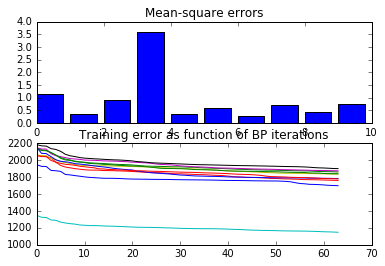
\includegraphics[width=0.7\textwidth]{Fig/regression_ANN_1.png}
	\vspace{-5pt}
	\caption{Selected features}
	\label{fig:selected_features}
\end{figure}

\vspace{-5pt}
%kommentar
\begin{figure}[!ht]
	\centering
	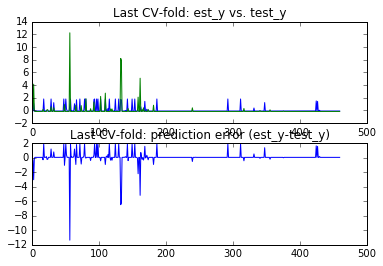
\includegraphics[width=0.7\textwidth]{Fig/regression_ANN_2.png}
	\vspace{-5pt}
	\caption{Comparing estimated values and test values, from the ANN}
	\label{fig:estimated_vs_test_values_ANN}
\end{figure}